\documentclass[tikz,border=10pt]{standalone}
\usepackage{amsmath}
\begin{document}

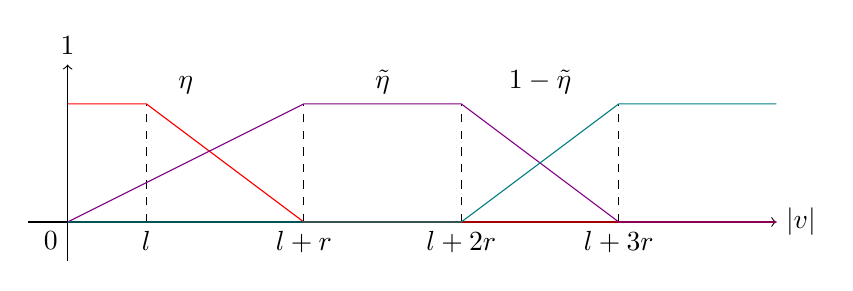
\begin{tikzpicture}
    % Colors
    \definecolor{color1}{rgb}{1,0,0}
    \definecolor{color2}{rgb}{0.5,0,0.5}
    \definecolor{color3}{rgb}{0,0.5,0.5}
    
    % Axes
    \draw[->] (-0.5,0) -- (9,0) node[right] {$|v|$};
    \draw[->] (0,-0.5) -- (0,2) node[above] {$1$};
    
    % Lines and labels
    \draw[dashed] (1,0) -- (1,1.5);
    \draw[dashed] (3,0) -- (3,1.5);
    \draw[dashed] (5,0) -- (5,1.5);
    \draw[dashed] (7,0) -- (7,1.5);
    
    \node[below] at (1,0) {$l$};
    \node[below] at (3,0) {$l + r$};
    \node[below] at (5,0) {$l + 2r$};
    \node[below] at (7,0) {$l + 3r$};
    
    % Functions
    \draw[color1] (0,1.5) -- (1,1.5) -- (3,0) -- (9,0);
    \node[above] at (1.5,1.5) {$\eta$};
    
    \draw[color2] (0,0) -- (3,1.5) -- (5,1.5) -- (7,0) -- (9,0);
    \node[above] at (4,1.5) {$\tilde \eta$};
    
    \draw[color3] (0,0) -- (5,0) -- (7,1.5) -- (9,1.5);
    \node[above] at (6,1.5) {$1-\tilde \eta$};
    
    % Origin label
    \node[below left] at (0,0) {$0$};
\end{tikzpicture}

\end{document}